%
% This is a borrowed LaTeX template file for lecture notes for CS267,
% Applications of Parallel Computing, UCBerkeley EECS Department.
% Now being used for CMU's 10725 Fall 2012 Optimization course
% taught by Geoff Gordon and Ryan Tibshirani.  When preparing 
% LaTeX notes for this class, please use this template.
%
% To familiarize yourself with this template, the body contains
% some examples of its use.  Look them over.  Then you can
% run LaTeX on this file.  After you have LaTeXed this file then
% you can look over the result either by printing it out with
% dvips or using xdvi. "pdflatex template.tex" should also work.
%
\documentclass[twoside]{article}
\usepackage{graphicx}
\usepackage{tikz}
\usepackage{mathpazo}
\usetikzlibrary{decorations.pathmorphing}


\setlength{\oddsidemargin}{0.25 in}
\setlength{\evensidemargin}{-0.25 in}
\setlength{\topmargin}{-0.6 in}
\setlength{\textwidth}{6.5 in}
\setlength{\textheight}{8.5 in}
\setlength{\headsep}{0.75 in}
\setlength{\parindent}{0 in}
\setlength{\parskip}{0.1 in}
%
% ADD PACKAGES here:
%
\usepackage{amsmath,amsfonts,graphicx}
%
% The following commands set up the lecnum (lecture number)
% counter and make various numbering schemes work relative
% to the lecture number.
%
\newcounter{lecnum}
\renewcommand{\thepage}{\thelecnum-\arabic{page}}
\renewcommand{\thesection}{\thelecnum.\arabic{section}}
\renewcommand{\theequation}{\thelecnum.\arabic{equation}}
\renewcommand{\thefigure}{\thelecnum.\arabic{figure}}
\renewcommand{\thetable}{\thelecnum.\arabic{table}}
%
% The following macro is used to generate the header.
%
\newcommand{\lecture}[5]{
   \pagestyle{myheadings}
   \thispagestyle{plain}
   \newpage
   \setcounter{lecnum}{#1}
   \setcounter{page}{1}
   \noindent
   \begin{center}
   \framebox{
      \vbox{\vspace{2mm}
    \hbox to 6.28in { {\bf Physics 467/667: Thermodynamics/Statistical Physics
	\hfill Spring 2017} }
       \vspace{4mm}
       \hbox to 6.28in { {\Large \hfill Lecture #1: #2  \hfill} }
       \vspace{2mm}
       \hbox to 6.28in { {\it Lecturer: #3 \hfill Scribes: #4} }
      \vspace{2mm}}
   }
   \end{center}
   \markboth{Lecture #1: #2}{Lecture #1: #2}
   \vspace*{4mm}
}
%
%
% Convention for citations is authors' initials followed by the year.
% For example, to cite a paper by Leighton and Maggs you would type
% \cite{LM89}, and to cite a paper by Strassen you would type \cite{S69}.
% (To avoid bibliography problems, for now we redefine the \cite command.)
% Also commands that create a suitable format for the reference list.
\renewcommand{\cite}[1]{[#1]}
\def\beginrefs{\begin{list}%
        {[\arabic{equation}]}{\usecounter{equation}
         \setlength{\leftmargin}{2.0truecm}\setlength{\labelsep}{0.4truecm}%
         \setlength{\labelwidth}{1.6truecm}}}
\def\endrefs{\end{list}}
\def\bibentry#1{\item[\hbox{[#1]}]}
%Use this command for a figure; it puts a figure in wherever you want it.
%usage: \fig{NUMBER}{SPACE-IN-INCHES}{CAPTION}
\newcommand{\fig}[3]{
			\vspace{#2}
			\begin{center}
			Figure \thelecnum.#1:~#3
			\end{center}
	}
% Use these for theorems, lemmas, proofs, etc.
\newtheorem{theorem}{Theorem}[lecnum]
\newtheorem{lemma}[theorem]{Lemma}
\newtheorem{proposition}[theorem]{Proposition}
\newtheorem{claim}[theorem]{Claim}
\newtheorem{corollary}[theorem]{Corollary}
\newtheorem{definition}[theorem]{Definition}
\newenvironment{proof}{{\bf Proof:}}{\hfill\rule{2mm}{2mm}}
% **** IF YOU WANT TO DEFINE ADDITIONAL MACROS FOR YOURSELF, PUT THEM HERE:
\newcommand\E{\mathbb{E}}
\begin{document}
%FILL IN THE RIGHT INFO.
%\lecture{**LECTURE-NUMBER**}{**DATE**}{**LECTURER**}{**SCRIBE**}
\lecture{9}{Entropy and Heat}{Qiang Zhu}{scribe-name1,2,3}
%\footnotetext{These notes are partially based on those of Nigel Mansell.}
% **** YOUR NOTES GO HERE:
% Some general latex examples and examples making use of the
% macros follow.  
%**** IN GENERAL, BE BRIEF. LONG SCRIBE NOTES, NO MATTER HOW WELL WRITTEN,
%**** ARE NEVER READ BY ANYBODY.

\section{Some useful equations} % Don't be this informal in your notes!
\begin{equation} \label{idealgas} PV = nRT = NkT \end{equation}
\begin{equation} \label{Avogadro} N = n \times N_A \end{equation}
\begin{equation} \label{PV-micro} PV = Nm{\overline v_x^2} = NkT\end{equation}
\begin{equation} \label{eqpartition} U_{thermal} = N \cdot f \cdot \frac{1}{2}kT \end{equation}
\begin{equation} \label{1stlaw} \Delta{U} = Q + W \end{equation}
\begin{equation} \label{work3} \Delta W = - P \Delta{V} \end{equation}
\begin{equation} \label{entropy} S = k \text{ln}\Omega \end{equation}

\section{Express Temperature with respect to Entropy}
Show that during the quasistatic isothermal expansion, the change of entropy is related to the heat input $Q$ by
\begin{equation} \label{entropy} 
\Delta{S}=\frac{Q}{T}     ~~~~~~~~ \rightarrow~~~~~~~~  T = \frac{Q}{\Delta{S}}
\end{equation}

It looks like $T$ is can expressed as energy divided by entropy.

\begin{figure}[ht]
\centering
\label{dS}
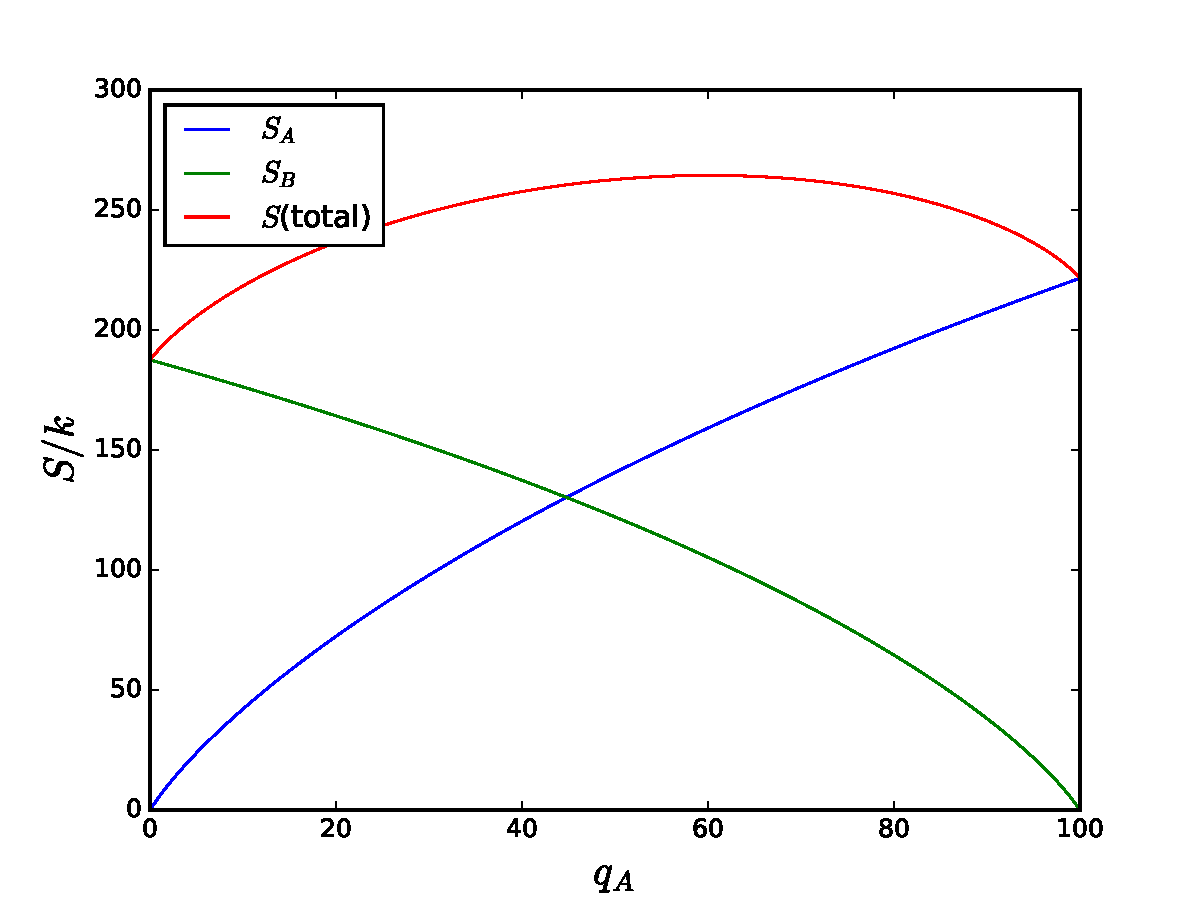
\includegraphics[width=9cm]{Einstein3}
\caption{ Entropy as a function of $q_A$ in two interacting Einstein solids ($N_A$=300, $N_B$=200, $q$(total)=100). }
\end{figure}


In the context of two interacting Einstein solid, we once calcluated $\Omega$ as a function of $q_A$. Let's redo it.
At equlibrium, we know $S_\text{total}$ reaches the maximum, therefore,
\begin{equation} \label{entropy} 
\frac {\partial{S_\text{total}}} {\partial{q_A}}=0     ~~~~~~~~ \rightarrow~~~~~~~~  \frac {\partial{S_\text{total}}} {\partial{U_A}}=0
\end{equation}

Since $S_\text{total}$ is simply the sum of $S_A$ and $S_B$, we now know
\begin{equation} \label{entropy} 
\frac {\partial{S_A}} {\partial{U_A}} +  \frac {\partial{S_B}} {\partial{U_A}} =0     ~~~~~~~~ \rightarrow~~~~~~~~  
\frac {\partial{S_A}} {\partial{U_A}} =  \frac {\partial{S_B}} {\partial{U_B}} 
\end{equation}

At the equilibrium, which quantity of $A$ and $B$ becomes equivalent. \\
The consequence of heat flow?\\
Check the unit! Yes, the slope of $S_A$ is acutally the reciprocal of $T$.\\
Therefore we have
\begin{equation} 
1/T = \frac {\partial{S}} {\partial{U}} ~~~~~~~~ \rightarrow~~~~~~~~ T = \frac {\partial{U}} {\partial{S}}.
\end{equation}

{\bf Exercise}\\
Calculate the slope of $S$-$q$ graph for various points. (assuming $\epsilon$=0.1eV, 0.024 eV is about 300 K, )\\
\begin{enumerate}
\item $q$=0,  $(\frac {\Delta{S_A}} {\Delta{U_A}})^{-1}$=  ~~~~~~~~~~~~~~~~~~~~~~~~~~~~~~  $(\frac {\Delta{S_B}} {\Delta{U_B}})^{-1}$= 
\item $q$=10, $(\frac {\Delta{S_A}} {\Delta{U_A}})^{-1}$=  ~~~~~~~~~~~~~~~~~~~~~~~~~~~~~~  $(\frac {\Delta{S_B}} {\Delta{U_B}})^{-1}$= 
\item $q$=60, $(\frac {\Delta{S_A}} {\Delta{U_A}})^{-1}$=  ~~~~~~~~~~~~~~~~~~~~~~~~~~~~~~  $(\frac {\Delta{S_B}} {\Delta{U_B}})^{-1}$= 
\end{enumerate}

\section{Einstein Solid}

\begin{equation} S = Nk[\text{ln}(q/N)+1] = Nk\text{ln}U - Nk\text{ln}(\epsilon N) + Nk \end{equation}
\begin{equation} T = (\frac {\partial{S}} {\partial{U}})^{-1} = (\frac{Nk}{U})^{-1}\end{equation}
\begin{equation} U = NkT \end{equation}
This is exactly the thermal equipartition theorem applied to Einstein Solid.

\section{Ideal Gas}

\begin{equation} S = Nk\text{ln}V + 3/2Nk\text{ln}U - Nk\text{ln}(f(N)) \end{equation}
\begin{equation} T = (\frac {\partial{S}} {\partial{U}}) ^{-1} = ~~~~~\end{equation}
\begin{equation} U = 3/2NkT \end{equation}


\section{Measuring Entropies}
\begin{equation} dS = \frac{dU}{T} = \frac{Q}{T}   ~~~~~~~~~~~~~~~~~ \text{(constant volume, W = 0)}\end{equation}
\begin{equation} dS = \frac{C_V}{T}   ~~~~~~~~~~~~~~~~~ \text{(constant volume, W = 0)}\end{equation}
\begin{equation} \Delta{S} = S_f-S_i = \int^{T_f}_{T_i} \frac{C_V}{T} dT \end{equation}
\begin{equation} \Delta{S} = \int^B_A \frac{C_V}{T} dT \end{equation}

What is $S$ when $T$=0, in principle $\Omega$=1, so $S$=0.\\
However, solid crystals have residual entropy due to the random orientations, so the configuration at 0K is not 1!
For instance, each CO molecule has two possible orientations: CO or OC. Assuming they are completely random, what's the residual entropy of 1 mole CO?\\\\
$S(0K)$ = $k$ln($\Omega$) = $k$ln$2^N$ = $Nk$ln2 = ~~~~~~~~~~~~~~~~~~~~~~~~~~~~~~~~ = 5.8 J/K\\
$S(300K)$ = $S(0K) + C_V \int^{300}_{0} \frac{1}{T} dT$ = 5.8 + 2.5*8.31*ln(300) = 5.8 + 118.50 = 124.30 J/K\\\\
This value looks much smaller than the reference value in the appendix (197.67 J/K), because of constant volume assumption is not realistic.

\section{Microscopic view}
\begin{figure}[h]
\centering
\begin{tikzpicture}[thick]
\draw (0,0.4) -- (8,0.4) -- (8,4) -- (0,4) -- (0,0.4);
\draw (0.2,0.6) -- (3.2,0.6) -- (3.2,3.8) -- (0.2,3.8) -- (0.2,0.6);
\node at (1.8,2.8) {Solid $A$};
\node at (1.8,2.2) {500 K};
\draw (7.8,0.6) -- (4.8,0.6) -- (4.8,3.8) -- (7.8,3.8) -- (7.8,0.6);
\node at (5.8,2.8) {Solid $B$};
\node at (5.8,2.2) {300 K};
\draw [->,decorate,decoration=snake] (3.2,2) -- (4.8,2) node [above, xshift=-1cm]{1500 J};
\end{tikzpicture}
\caption{A schematic heat flow between two interacting Einstein solids.}
\end{figure}
\begin{enumerate}
\item Object $A$ loses entropy by $dQ/T$ = -3 J/K 
\item Object $B$ gain  entropy by $dQ/T$ = +5 J/K 
\item The total entropy increases by +2 J/K
\item Fundamentally, the net increase in entropy is the driving force behind the flow of heat.
\item The manifestation of 2nd law
\end{enumerate}

\section{Homework}
Problem 3.5, 3.8, 3.11, 3.14, 3.16
\end{document}

